\documentclass[12pt,a4paper]{article}
\usepackage[utf8]{inputenc}
\usepackage[margin=1in]{geometry}
\usepackage{graphicx}
\usepackage{hyperref}
\usepackage{listings}
\usepackage{xcolor}
\usepackage{enumitem}
\usepackage{float}
\usepackage{tikz}
\usetikzlibrary{shapes.geometric, arrows}

% TikZ styles for flowchart
\tikzstyle{startstop} = [rectangle, rounded corners, minimum width=3cm, minimum height=1cm, text centered, draw=black, fill=red!30]
\tikzstyle{process} = [rectangle, minimum width=3cm, minimum height=1cm, text centered, draw=black, fill=blue!30]
\tikzstyle{decision} = [diamond, aspect=2, minimum width=3cm, minimum height=1cm, text centered, draw=black, fill=green!30]
\tikzstyle{arrow} = [thick,->,>=stealth]

% Code listing setup
\definecolor{codegreen}{rgb}{0,0.6,0}
\definecolor{codegray}{rgb}{0.5,0.5,0.5}
\definecolor{codepurple}{rgb}{0.58,0,0.82}
\definecolor{backcolour}{rgb}{0.95,0.95,0.95}

\lstdefinestyle{javastyle}{
    backgroundcolor=\color{backcolour},   
    commentstyle=\color{codegreen},
    keywordstyle=\color{blue},
    numberstyle=\tiny\color{codegray},
    stringstyle=\color{codepurple},
    basicstyle=\ttfamily\footnotesize,
    breakatwhitespace=false,         
    breaklines=true,                 
    captionpos=b,                    
    keepspaces=true,                 
    numbers=left,                    
    numbersep=5pt,                  
    showspaces=false,                
    showstringspaces=false,
    showtabs=false,                  
    tabsize=2
}

\lstset{style=javastyle}

\title{\textbf{Design of a Chat Application Using\\Multi-threaded Socket Programming}}
\author{H.M. Mehedi Hasan (Roll: 13) \\ MD. Abu Bakar Siddique (Roll: 47)}
\date{\today}

\begin{document}

\maketitle
\tableofcontents
\newpage

\section{Introduction}

Socket programming is a fundamental technique that allows communication between processes over a network through endpoints called sockets. It forms the interface between application processes and the transport layer protocols such as TCP and UDP. This method is crucial in networked applications like chat systems where data exchange between clients and servers is constant and interactive.

Multi-threaded socket programming extends basic socket communication by employing multiple threads on the server side, enabling simultaneous handling of multiple clients. Each client is served by a dedicated thread that manages its connection independently. This concurrency is crucial for chat applications where multiple users interact in real time; it prevents blocking that occurs in basic single-threaded socket servers, thus ensuring responsiveness and scalability.

Without multi-threading, a server using basic socket programming can accept and communicate with only one client at a time, causing other client requests to wait indefinitely—making it impractical for chat applications.



\section{Objectives}

\begin{enumerate}
    \item To understand the core concepts of socket programming and the necessity of multi-threading.
    
    \item To design and implement a multi-threaded chat server that can simultaneously serve multiple clients.
    
    \item To enable continuous bi-directional communication where clients can send multiple messages and receive replies concurrently.
\end{enumerate}

\section{Design Details}

\subsection{Implementation Process}

\begin{enumerate}
    \item \textbf{Server Setup:}
    \begin{enumerate}
        \item The server creates a \texttt{ServerSocket} listening on port \texttt{3000}.
        \item It continuously accepts new client connections.
    \end{enumerate}

    \item \textbf{Client Connection Handling:}
    \begin{enumerate}
        \item Upon client connection, the server creates input and output streams (\texttt{DataInputStream} and \texttt{DataOutputStream}).
        \item A new thread (\texttt{ClientHandlerThread}) is spawned for each client, passing the socket and streams.
        \item The thread is responsible for communicating exclusively with its associated client.
    \end{enumerate}

    \item \textbf{ClientHandlerThread Details:}
    \begin{enumerate}
        \item Reads the client’s name upon joining.
        \item Continuously listens for messages from the client.
        \item If the client sends \texttt{"quit"}, the thread closes the connection and removes itself from the active client list.
        \item Broadcasts messages received from the client to all other connected clients.
    \end{enumerate}

    \item \textbf{Client Setup:}
    \begin{enumerate}
        \item The client connects to the server using the IP \texttt{localhost} and port \texttt{3000}.
        \item Sends its user name immediately after connecting.
        \item Has two threads:
        \begin{enumerate}
            \item One for reading user input and sending messages to the server.
            \item One for listening to incoming messages from the server and displaying them.
        \end{enumerate}
        \item The client terminates when the user types \texttt{"quit"}.
    \end{enumerate}
\end{enumerate}

\newpage
\subsection{Implementation Process (Flowchart)}

\begin{figure}[H]
\centering
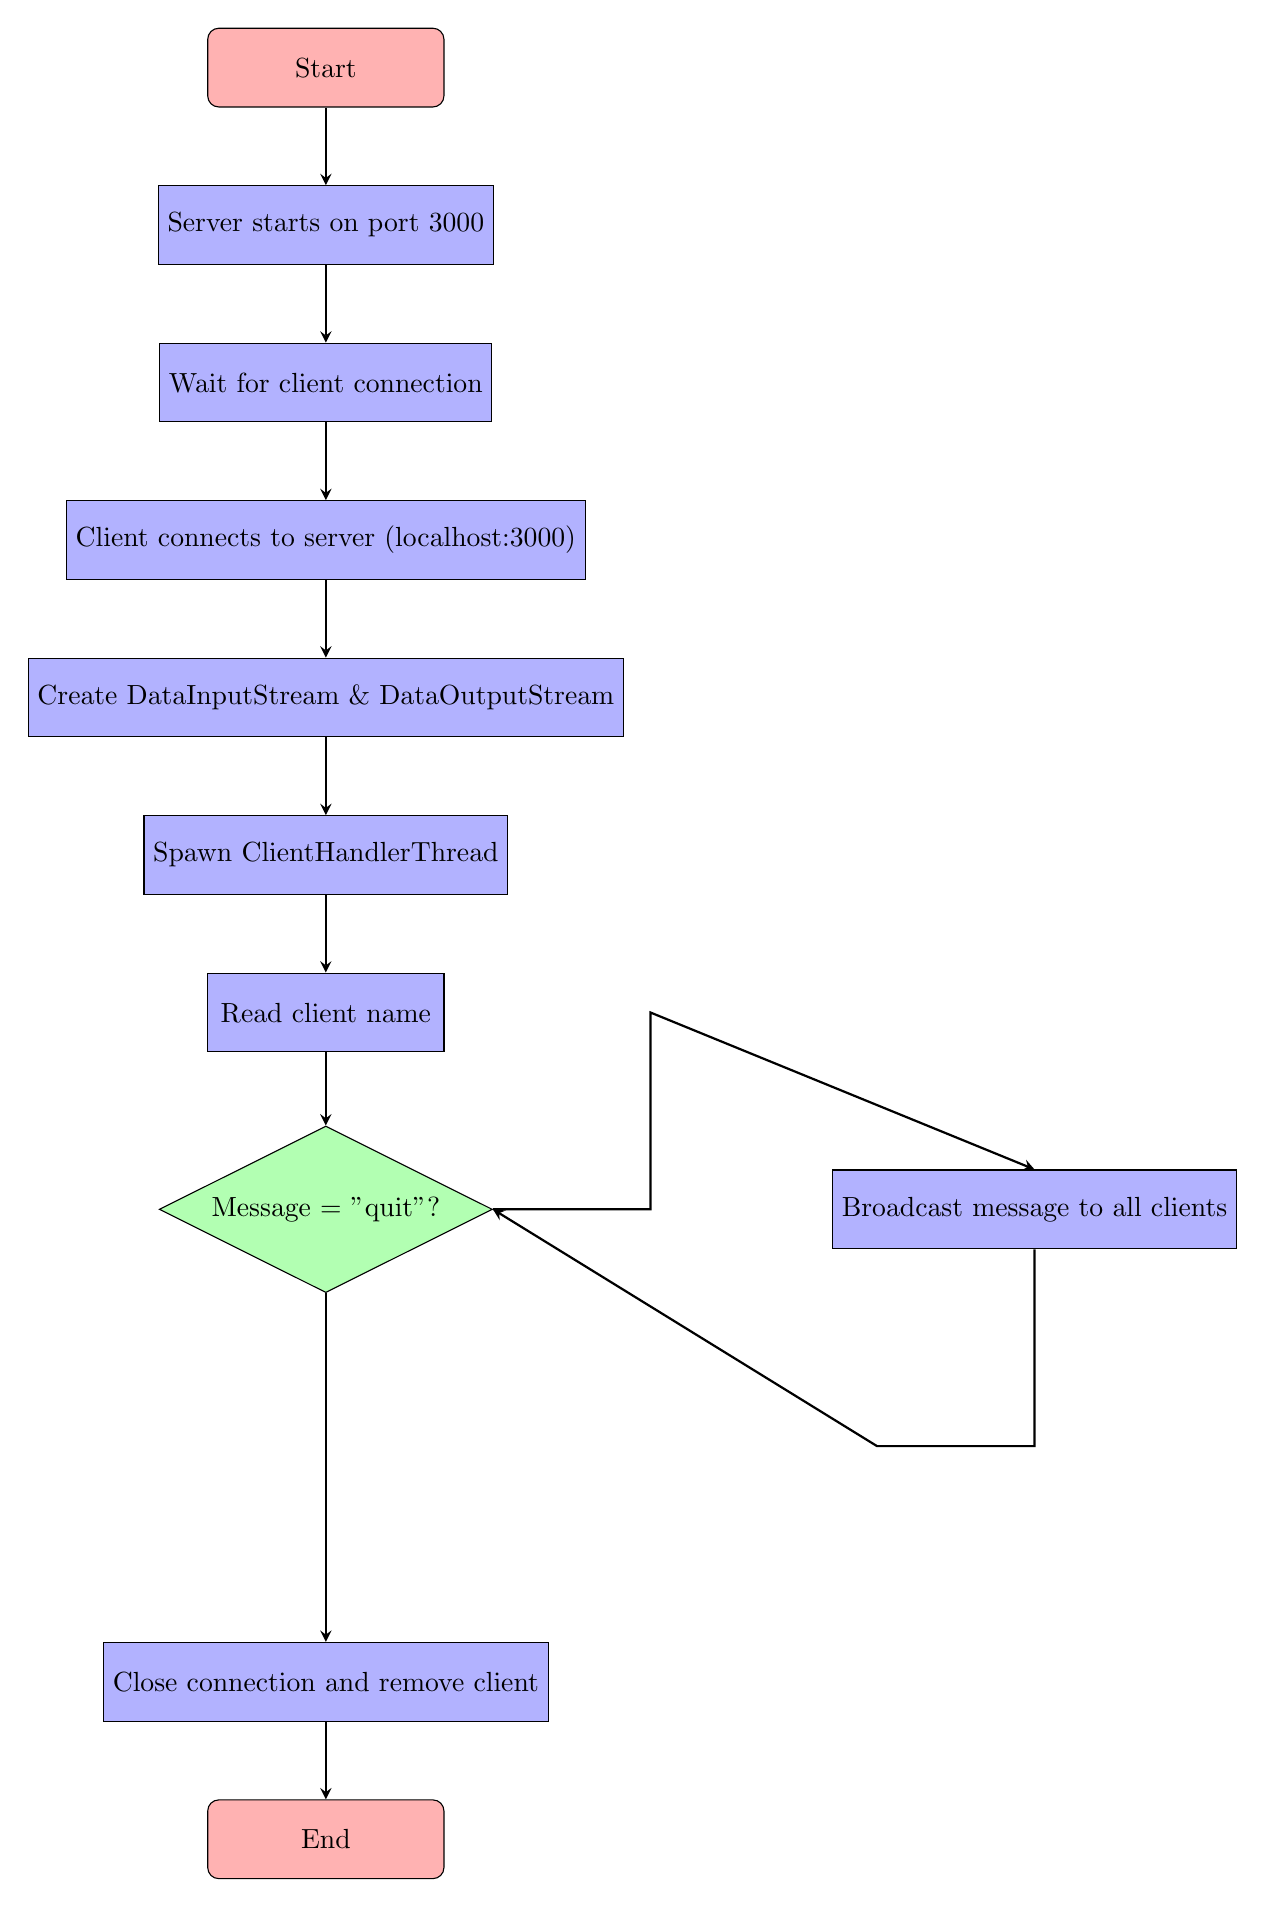
\begin{tikzpicture}[node distance=2cm]

% Nodes
\node (start) [startstop] {Start};
\node (server) [process, below of=start] {Server starts on port 3000};
\node (wait) [process, below of=server] {Wait for client connection};
\node (clientconnect) [process, below of=wait] {Client connects to server (localhost:3000)};
\node (streams) [process, below of=clientconnect] {Create DataInputStream \& DataOutputStream};
\node (thread) [process, below of=streams] {Spawn ClientHandlerThread};
\node (readname) [process, below of=thread] {Read client name};
\node (decision1) [decision, below of=readname, yshift=-0.5cm] {Message = "quit"?};
\node (broadcast) [process, right of=decision1, xshift=7cm] {Broadcast message to all clients};
\node (close) [process, below of=decision1, yshift=-4cm] {Close connection and remove client};
\node (end) [startstop, below of=close] {End};

% Arrows
\draw [arrow] (start) -- (server);
\draw [arrow] (server) -- (wait);
\draw [arrow] (wait) -- (clientconnect);
\draw [arrow] (clientconnect) -- (streams);
\draw [arrow] (streams) -- (thread);
\draw [arrow] (thread) -- (readname);
\draw [arrow] (readname) -- (decision1);
\draw [arrow] (decision1.east) -- ++(2,0) -- ++(0,2.5) -- (broadcast.north);
\draw [arrow] (broadcast.south) -- ++(0,-2.5) -- ++(-2,0) -- (decision1.east);
\draw [arrow] (decision1.south) -- (close.north);
\draw [arrow] (close.south) -- (end.north);

\end{tikzpicture}
\caption{Server Implementation Flowchart}
\label{fig:flowchart}
\end{figure}

\section{Implementation}

The implementation consists of two main Java classes: Server.java and Client.java. Below are the key components of each:

\subsection{Server Implementation}

\begin{lstlisting}[language=Java, caption=Server.java - Main Server Class]

import java.io.DataInputStream;
import java.io.DataOutputStream;
import java.net.ServerSocket;
import java.net.Socket;
import java.util.Scanner;
import java.util.Vector;

public class Server_13_47 {
    public static Vector<ClientHandlerThread> clientThreads = new Vector<>();
    public static int selectedIndex = 0;

    public static void main(String[] args) throws Exception {

        ServerSocket ss = new ServerSocket(3000);
        System.out.println("New Server Created");
        Scanner sc = new Scanner(System.in);
        new Thread(() -> {
            try {
                while (true) {
                    Socket s = ss.accept();

                    DataInputStream in = new DataInputStream(s.getInputStream());
                    DataOutputStream out = new DataOutputStream(s.getOutputStream());

                    ClientHandlerThread thread = new ClientHandlerThread(s, in, out, clientThreads.size());
                    clientThreads.add(thread);

                    thread.start();
                }
            } catch (Exception e) {
               System.out.println("Error in accepting client" + e);
            }

        }).start();

        new Thread(() -> {
            try {
                while (true) {
                    System.out.print("\033[H\033[2J");
                    System.out.flush();

                    System.out.println("0. Exit");
                    String read = sc.nextLine();
                    if (read.equals("0")) {
                        System.out.println("Quitting...");
                        System.exit(0);
                        break;
                    }

                }
            } catch (Exception e) {
                System.out.println("Error in i/o thread");
            }

        }).start();

    }
}

class ClientHandlerThread extends Thread {
    public Socket s;
    DataInputStream in;
    DataOutputStream out;
    String name;
    Vector<ClientHandlerThread> clientList;

    public ClientHandlerThread(Socket s, DataInputStream in, DataOutputStream out, int index) {
        this.s = s;
        this.in = in;
        this.out = out;
        this.clientList = Server_13_47.clientThreads;
    }

    @Override
    public void run() {
        try {
           
            name = in.readUTF();
            System.out.println(name + " joined the server!");
            
            while (true) {
                String message = in.readUTF();
                
                if (message.equals("quit")) {
                    System.out.println(name + " left the server!");
                    break;
                }
                
                broadcastMessage(name + ": " + message, this);
            }
            
        } catch (Exception e) {
            System.out.println(name + " disconnected unexpectedly");
        } finally {
            clientList.remove(this);
            try {
                s.close();
            } catch (Exception e) {
                System.out.println("Error closing socket");
            }
        }
    }
  
    private void broadcastMessage(String message, ClientHandlerThread sender) {
        for (ClientHandlerThread client : clientList) {
            if (client != sender) {
                try {
                    client.out.writeUTF(message);
                } catch (Exception e) {
                    System.out.println("Failed to send message to " + client.name);
                }
            }
        }
    }

}
\end{lstlisting}

\subsection{Client Implementation}

\begin{lstlisting}[language=Java, caption=Client.java - Main Client Class]
import java.io.DataInputStream;
import java.io.DataOutputStream;
import java.net.Socket;
import java.util.Scanner;
import java.util.concurrent.atomic.AtomicBoolean;

public class Client_13_47 {
    public static void main(String[] args) throws Exception {

        System.out.print("\033[H\033[2J");
        System.out.flush();
        Scanner sc = new Scanner(System.in);
        
        String name = "";
        
        System.out.print("Enter Name:");
        name = sc.nextLine();
        
        Socket s = new Socket("localhost", 3000);
        DataOutputStream out = new DataOutputStream(s.getOutputStream());
        DataInputStream in = new DataInputStream(s.getInputStream());

        System.out.println("Joined Server: "+ name);
        System.out.print("\033[H\033[2J");
        System.out.flush();
        System.out.println("Welcome " + name + "!");
        System.out.println("Type your messages below. Type 'quit' to exit.");
        out.writeUTF(name);
        AtomicBoolean running = new AtomicBoolean(true);
        new Thread(() -> {
            try {
                while (running.get()) {
                    String message = sc.nextLine();
                    if (message.equals("quit")) {
                        running.set(false);
                        out.writeUTF(message);
                        break;
                    }
                    if (!message.trim().isEmpty()) {
                        System.out.println("You: " + message);
                        out.writeUTF(message);
                    }
                }
            } catch (Exception e) {
                System.out.println("Error sending message");
            }
        }).start();

        new Thread(() -> {
            try {
                while (running.get()) {
                    String message = in.readUTF();
                    System.out.println(message);
                }
            } catch (Exception e) {
                if (running.get()) {
                    System.out.println("Connection to server lost");
                }
            }
        }).start();
    }
}
\end{lstlisting}

\section{Result Analysis}

The implemented chat application successfully demonstrates the principles of multi-threaded socket programming, allowing for real-time communication between a server and multiple clients.

\subsection{Server Output}

\begin{figure}[H]
    \centering
    \includegraphics[width=1\linewidth]{server_output.png}
    \caption{Server Output}
    \label{fig:server_output}
\end{figure}

The server console displays:
\begin{itemize}
    \item Listens on port 3000.
    \item Manages all connected clients in a thread-safe Vector.
    \item Spawns a dedicated ClientHandlerThread per client.
    \item Supports broadcasting messages to multiple clients.
    \item Provides a console interface to exit the server.
\end{itemize}

\subsection{Client Output}

\begin{figure}[H]
    \centering
    \includegraphics[width=1\linewidth]{Client 1 Ouput.png}
    \caption{Client 1 Output}
    \label{fig:client1_output}
\end{figure}

\begin{figure}[H]
    \centering
    \includegraphics[width=1\linewidth]{Client 2 Output.png}
    \caption{Client 2 Output}
    \label{fig:client2_output}
\end{figure}

The client console displays:
\begin{itemize}
    \item Connects to server at localhost port 3000.
    \item Sends user name to server on connect.
    \item Runs two threads:
        \begin{itemize}
            \item For sending messages input by the user.
            \item For receiving and printing messages from server.
        \end{itemize}
    \item Supports sending multiple messages asynchronously.
    \item Stops on user input "quit".
\end{itemize}



\section{Discussion}

In this project, we explored both basic socket programming and multi-threaded socket programming. The comparison between the two approaches highlights the advantages and drawbacks of each.

\subsection{Basic Socket Programming}
\begin{itemize}
    \item In basic socket programming, a server can handle only one client at a time. 
    \item The server must wait for the current client to disconnect before accepting a new connection. 
    \item This approach is simple to implement but becomes impractical when multiple clients need to communicate simultaneously. 
    \item The main drawback is that client requests are processed sequentially, which may cause delays and poor performance.
\end{itemize}

\subsection*{Multi-Threaded Socket Programming}
\begin{itemize}
    \item In multi-threaded socket programming, a new thread is spawned for each connected client. 
    \item This allows the server to handle multiple clients concurrently without blocking other connections. 
    \item It improves responsiveness and scalability, as clients can send and receive messages independently. 
    \item Although this introduces additional complexity in managing threads and shared resources, the overall performance and user experience are significantly better.
\end{itemize}

\subsection*{Overcoming the Drawbacks}
\begin{itemize}
    \item The limitations of basic socket programming, such as sequential client handling and poor scalability, are overcome by using multi-threading. 
    \item With this program, we were able to broadcast messages from one client to all others efficiently, which would not be feasible in a single-threaded setup. 
    \item Thread-based design ensures that a single client’s disconnection or delay does not affect the entire server’s operation.
\end{itemize}

\subsection*{Learning Outcomes}
\begin{itemize}
    \item We learned how to establish socket connections and exchange data using input and output streams. 
    \item The project gave us hands-on experience with creating and managing threads in a networked environment. 
    \item We also gained insights into concurrency issues, synchronization, and resource management in multi-threaded systems.
\end{itemize}

\subsection*{Challenges Faced}
\begin{itemize}
    \item Understanding how to properly manage multiple threads was a significant challenge, especially when handling simultaneous client messages. 
    \item Ensuring that the server does not crash when a client abruptly disconnects required careful exception handling. 
    \item Debugging concurrent code was more complex compared to basic socket programming. 
    \item Despite these difficulties, the process enhanced our understanding of both networking and multithreading concepts.
\end{itemize}



\end{document}